\documentclass[12pt,a4paper]{article}

\usepackage[utf8]{inputenc}
\usepackage[english]{babel}
\usepackage{graphicx}
\usepackage{float}
\usepackage{amsmath}
\usepackage{hyperref}
\usepackage{listings}
\usepackage{xcolor}
\usepackage{booktabs}
\usepackage{subcaption}
\usepackage[margin=1in]{geometry}
\usepackage{cite}

\lstset{
    basicstyle=\ttfamily\small,
    keywordstyle=\color{blue},
    commentstyle=\color{green!60!black},
    stringstyle=\color{red},
    numbers=left,
    numberstyle=\tiny\color{gray},
    stepnumber=1,
    numbersep=5pt,
    backgroundcolor=\color{white},
    showspaces=false,
    showstringspaces=false,
    showtabs=false,
    frame=single,
    tabsize=2,
    captionpos=b,
    breaklines=true,
    breakatwhitespace=false,
    escapeinside={\%*}{*)},
    language=C++
}

\title{Real-time video processing\\
\large Visual Computing Assignment}
\author{Mads Pagh\\
Student ID: 202208375\\
Aarhus University}
\date{\today}

\begin{document}

\maketitle
\newpage

\tableofcontents
\newpage

\section{Introduction}
In this report an analysis of real-time image processing performance using OpenCV and OpenGL is presented. The project implements various image filters and geometric transformations, comparing CPU and GPU execution across different resolutions.

\subsection{Objectives}
\begin{itemize}
    \item Implement real-time image filters using OpenCV (CPU) and OpenGL shaders (GPU)
    \item Compare performance between CPU and GPU execution
    \item Analyze the impact of resolution on processing performance
    \item Evaluate the overhead of geometric transformations
\end{itemize}

\section{Methodology}

\subsection{System Architecture}
The system consists of three main components:
\begin{itemize}
    \item \textbf{Video Capture}: OpenCV VideoCapture for webcam input
    \item \textbf{Processing Pipeline}: CPU (OpenCV) and GPU (OpenGL/GLFW) implementations
    \item \textbf{Rendering}: OpenGL for display and GPU acceleration
\end{itemize}

\subsection{Implemented Filters}
Six different image filters were implemented:
\begin{enumerate}
    \item \textbf{None} - The frames are passed through without any filtering
    \item \textbf{Grayscale} - Color to grayscale conversion
    \item \textbf{Gaussian Blur} - 5x5 kernel blur
    \item \textbf{Edge Detection} - Sobel operator
    \item \textbf{Pixelation} - 10x10 pixel blocks
    \item \textbf{Comic Art} - Edge detection combined with color quantization
\end{enumerate}

\subsection{Geometric Transformations}
Five transformation configurations were tested:
\begin{enumerate}
    \item No Transform (baseline)
    \item Translation only ($t_x = 0.3, t_y = 0.2$)
    \item Scale only ($s = 1.5$)
    \item Rotation only ($\theta = 25 \text{ degrees}$)
    \item Combined ($t_x = 0.2, t_y = -0.15, s = 1.3, \theta = 15 \text{ degrees}$)
\end{enumerate}

\subsection{Test Resolutions}
Three resolutions were benchmarked:
\begin{itemize}
    \item VGA: 640×480 (307,200 pixels)
    \item HD: 1280×720 (921,600 pixels)
    \item Full HD: 1920×1080 (2,073,600 pixels)
\end{itemize}

\subsection{Benchmarking Procedure}
\begin{itemize}
    \item Each test configuration ran for 300 frames (transforms) or 50 frames (resolution)
    \item Frame times were measured using high-resolution clock
    \item Average FPS and frame time statistics were calculated
    \item Tests were automated to ensure consistency
\end{itemize}

\section{Results}

\subsection{Transform Benchmark Results}

\subsubsection{GPU vs CPU Performance}
\begin{figure}[H]
    \centering
    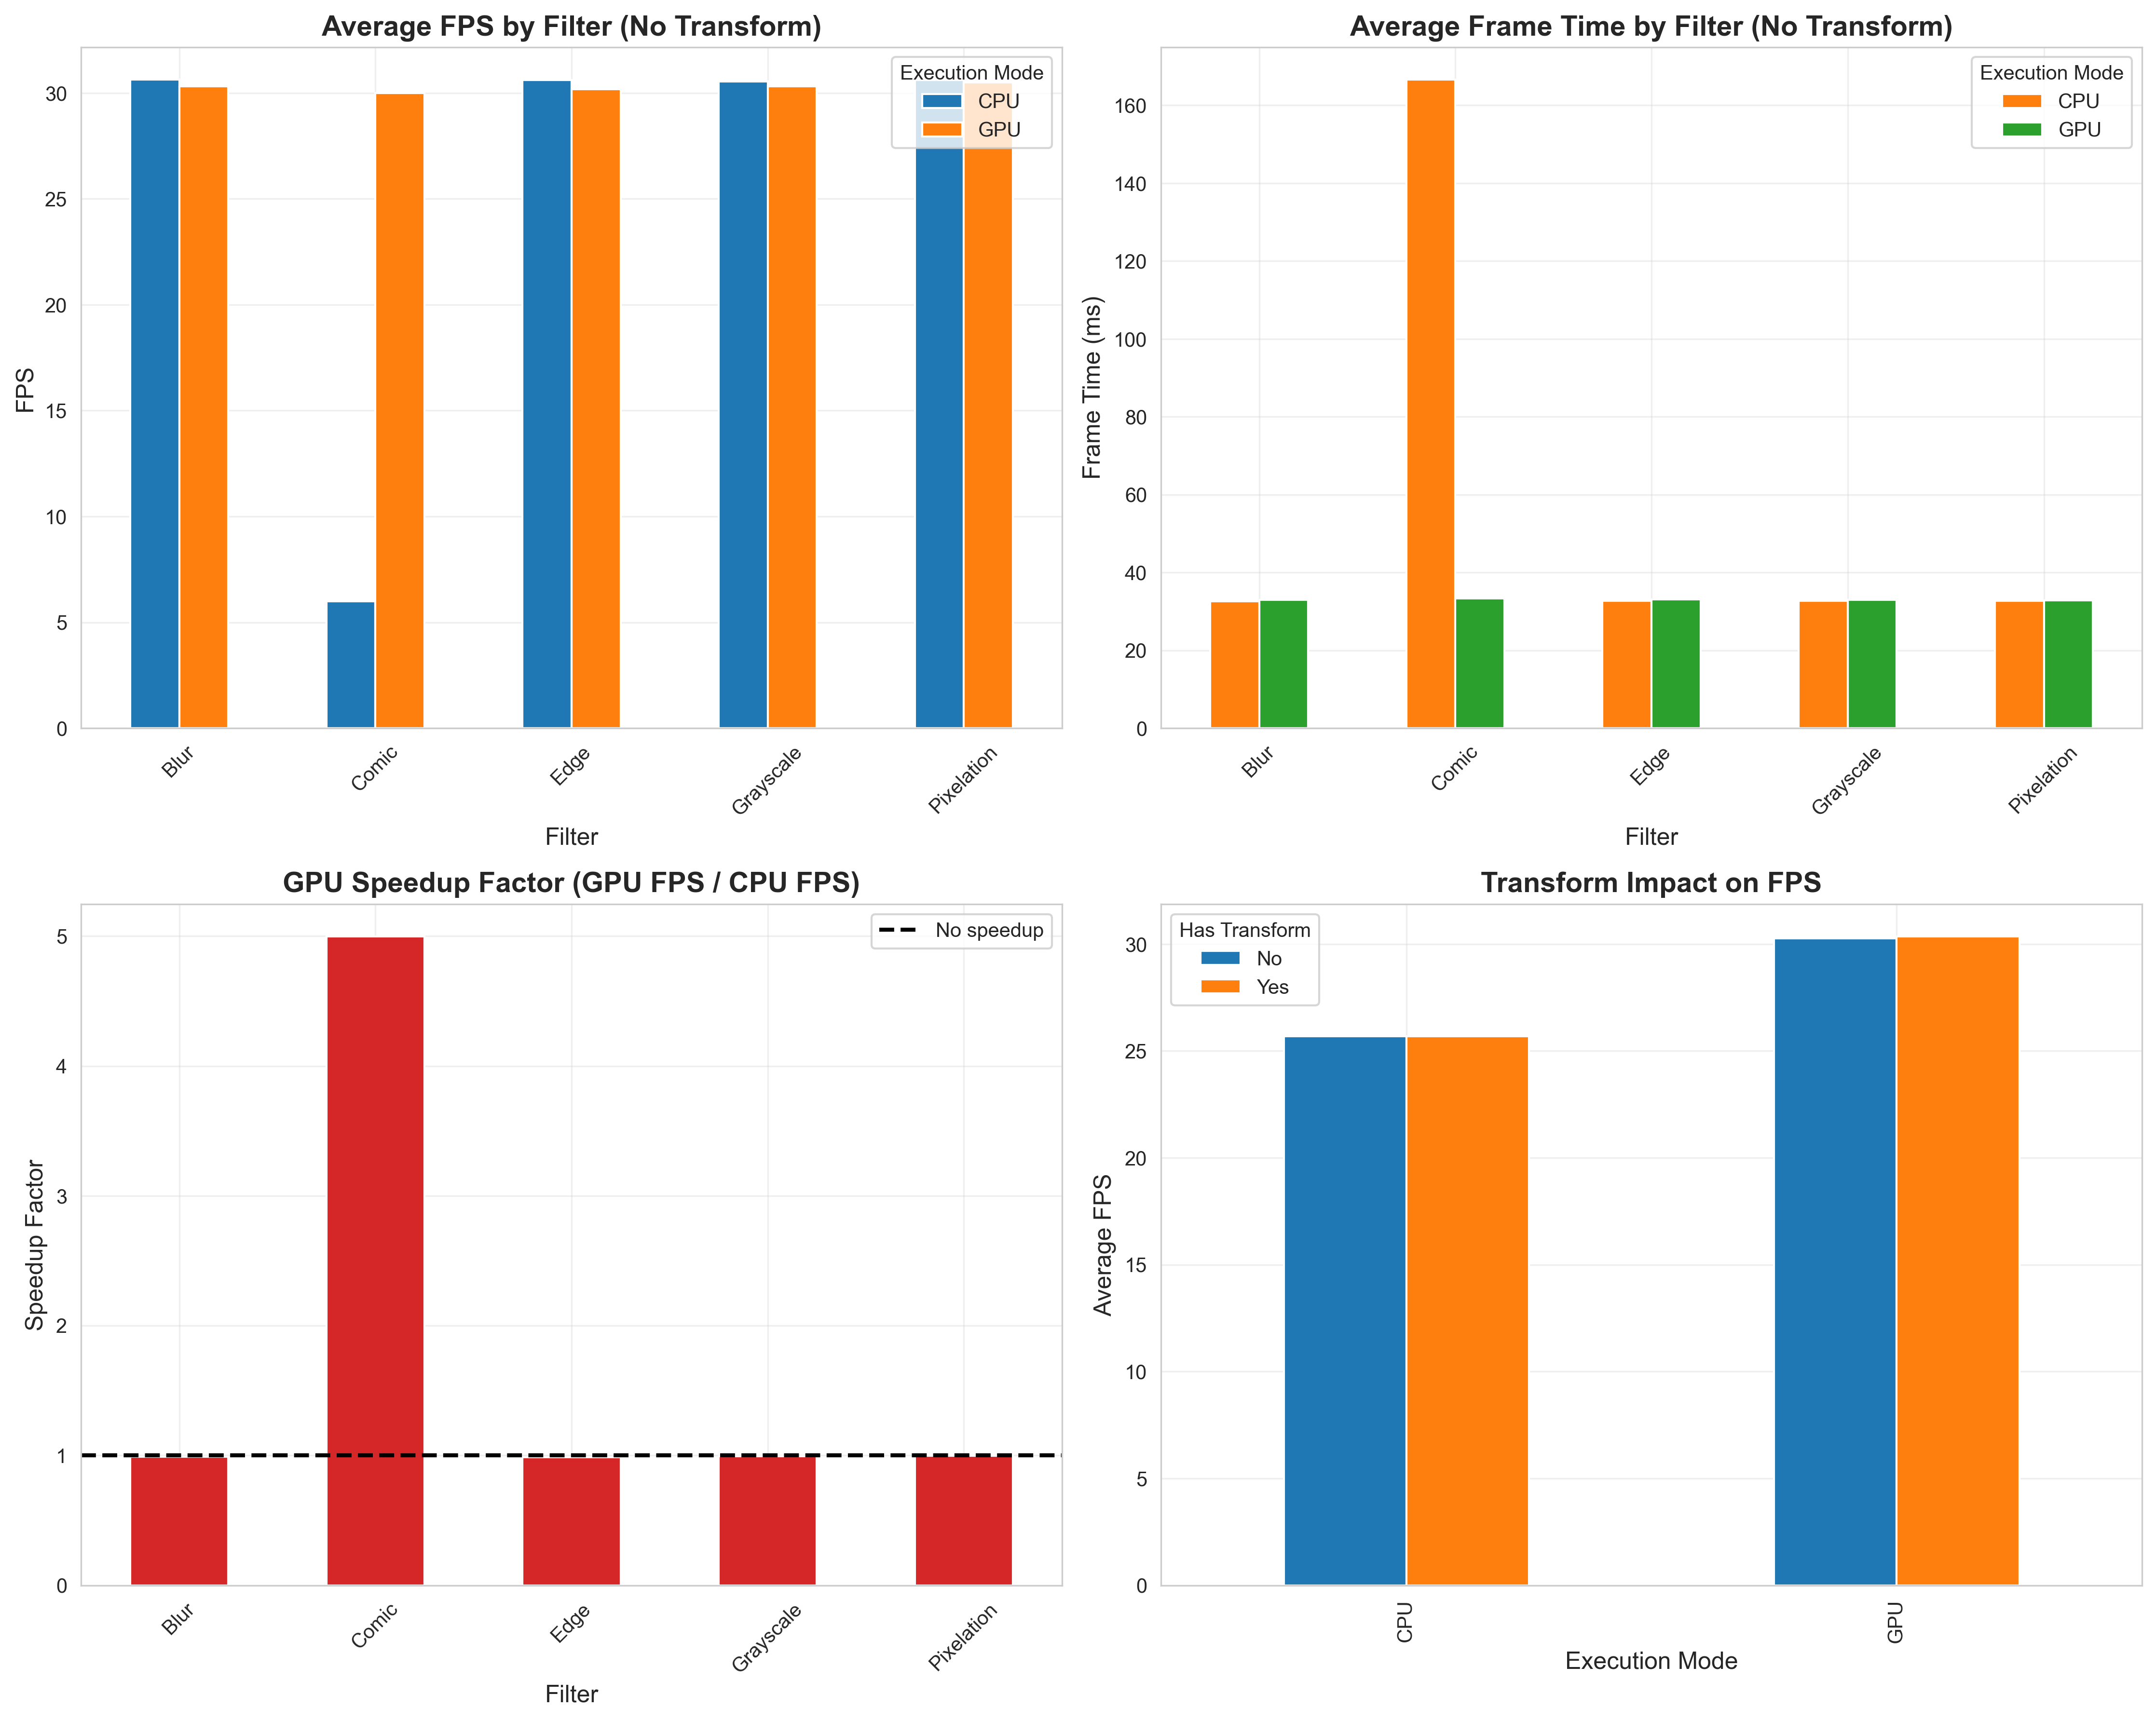
\includegraphics[width=0.9\textwidth]{../data/plots/performance_comparison_transforms.png}
    \caption{Performance comparison across filters and execution modes}
    \label{fig:transform_comparison}
\end{figure}

% TODO: Add analysis text here

\subsubsection{Transform Impact}
\begin{figure}[H]
    \centering
    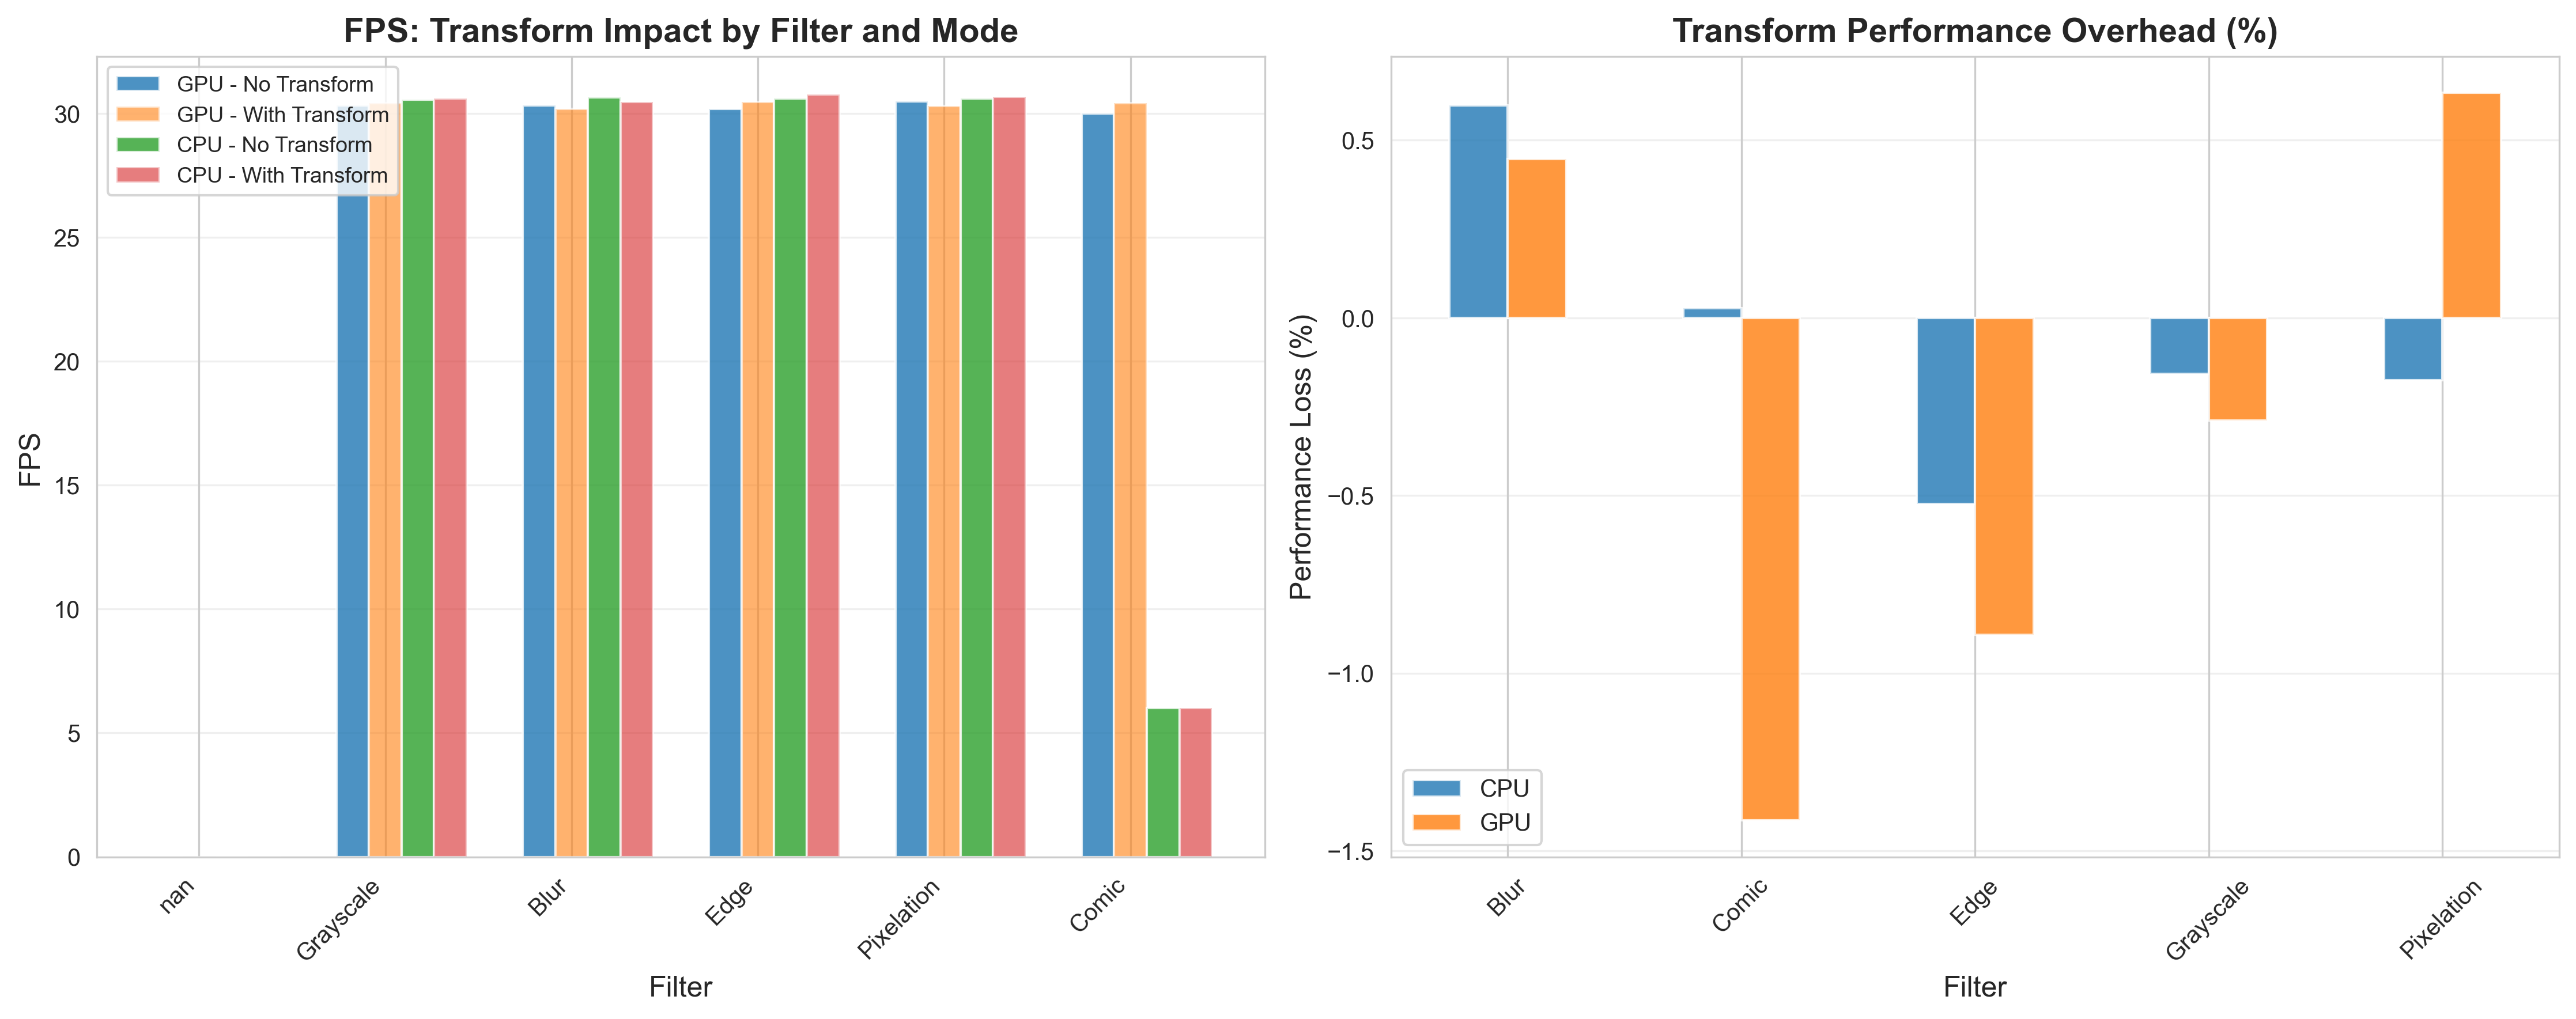
\includegraphics[width=0.9\textwidth]{../data/plots/transform_comparison.png}
    \caption{Impact of geometric transformations on performance}
    \label{fig:transform_impact}
\end{figure}

% TODO: Add analysis text here

\subsection{Resolution Benchmark Results}

\subsubsection{Resolution Scaling}
\begin{figure}[H]
    \centering
    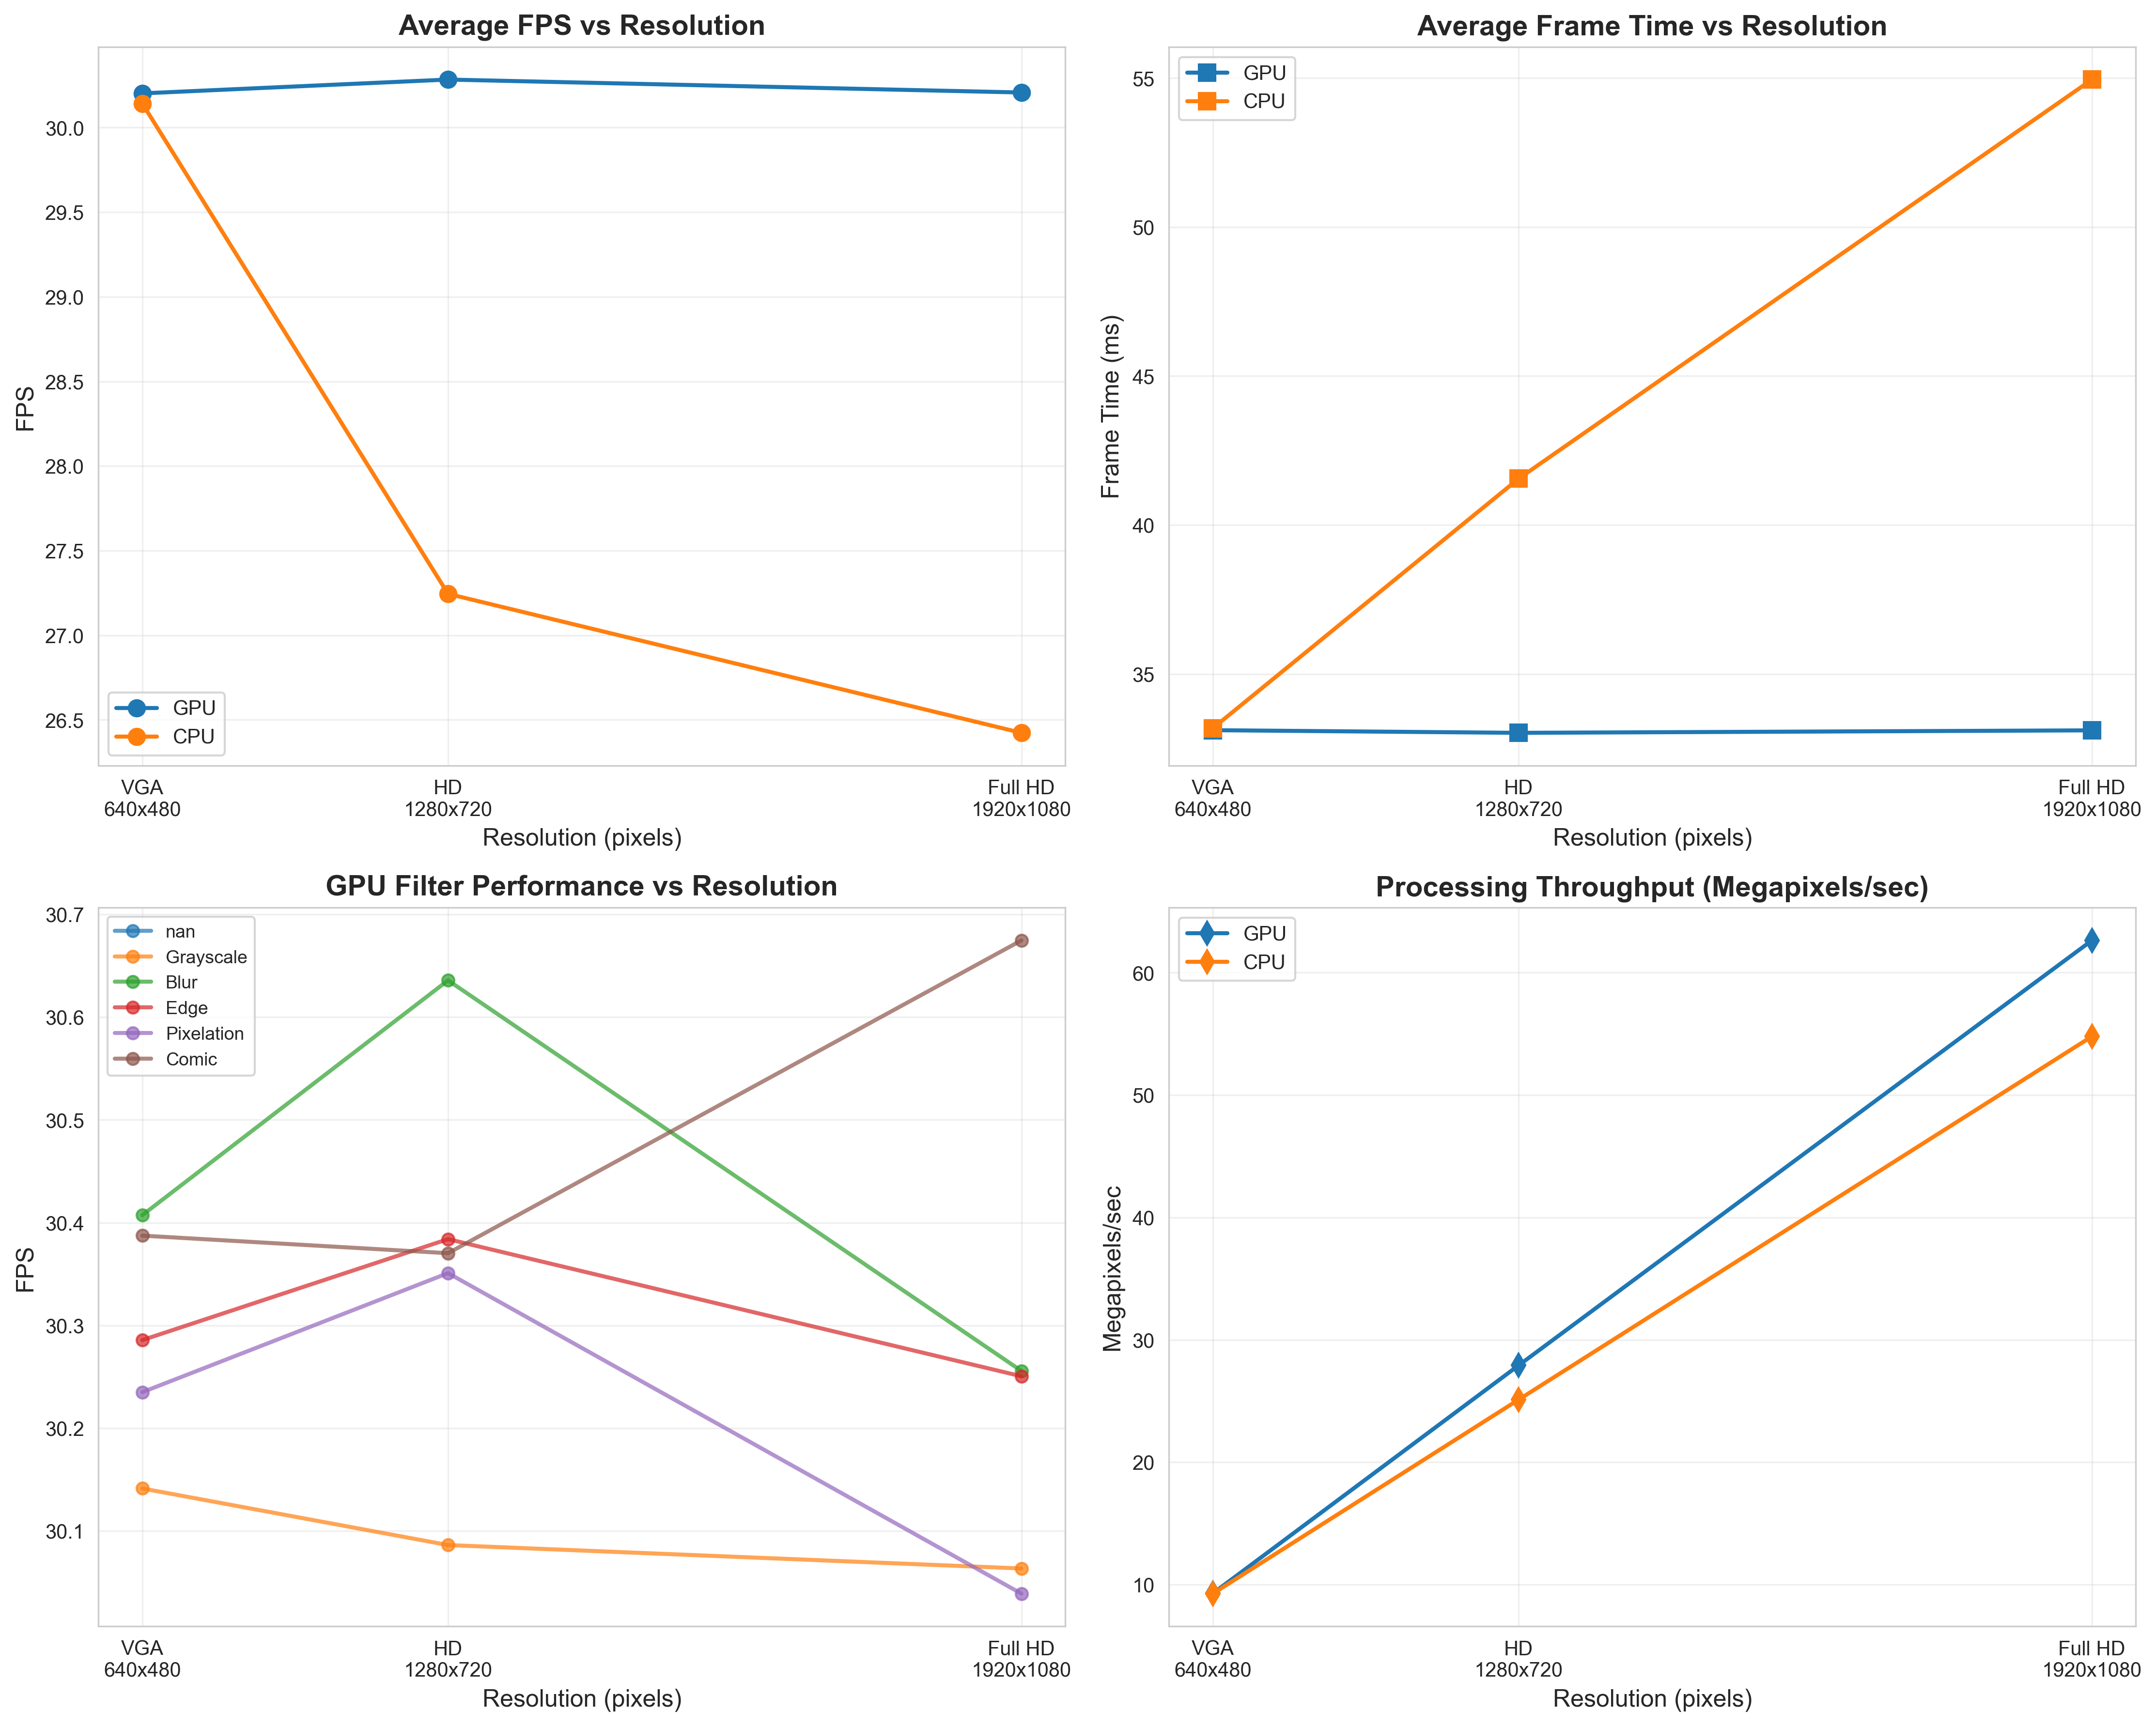
\includegraphics[width=0.9\textwidth]{../data/plots/resolution_impact.png}
    \caption{Performance across different resolutions}
    \label{fig:resolution_impact}
\end{figure}

% TODO: Add analysis text here

\subsection{Performance Tables}

\subsubsection{GPU Speedup Factors}
\begin{table}[H]
    \centering
    \caption{GPU speedup over CPU for each filter}
    \label{tab:speedup}
    \begin{tabular}{lc}
        \toprule
        Filter & Speedup Factor \\
        \midrule
        None & X.XX× \\
        Grayscale & X.XX× \\
        Blur & X.XX× \\
        Edge Detection & X.XX× \\
        Pixelation & X.XX× \\
        Comic Art & X.XX× \\
        \bottomrule
    \end{tabular}
\end{table}

% TODO: Import actual data from CSV files

\section{Analysis and Discussion}

\subsection{CPU vs GPU Performance}
% TODO: Discuss the performance differences between CPU and GPU

\subsection{Filter Complexity}
% TODO: Analyze how filter complexity affects performance

\subsection{Resolution Impact}
% TODO: Discuss how resolution affects both CPU and GPU performance

\subsection{Transform Overhead}
% TODO: Analyze the cost of geometric transformations

\subsection{Practical Implications}
% TODO: Discuss when to use CPU vs GPU processing

\section{Conclusion}
% TODO: Summarize key findings and conclusions

\subsection{Future Work}
Potential improvements and extensions:
\begin{itemize}
    \item Implement additional filters (bilateral, morphological operations)
    \item Test on different hardware configurations
    \item Optimize shader code for better GPU utilization
    \item Implement real-time performance adaptation
\end{itemize}

\bibliographystyle{plain}
\bibliography{references}

\end{document}